\documentclass{standalone}
\usepackage{tikz}

\begin{document}

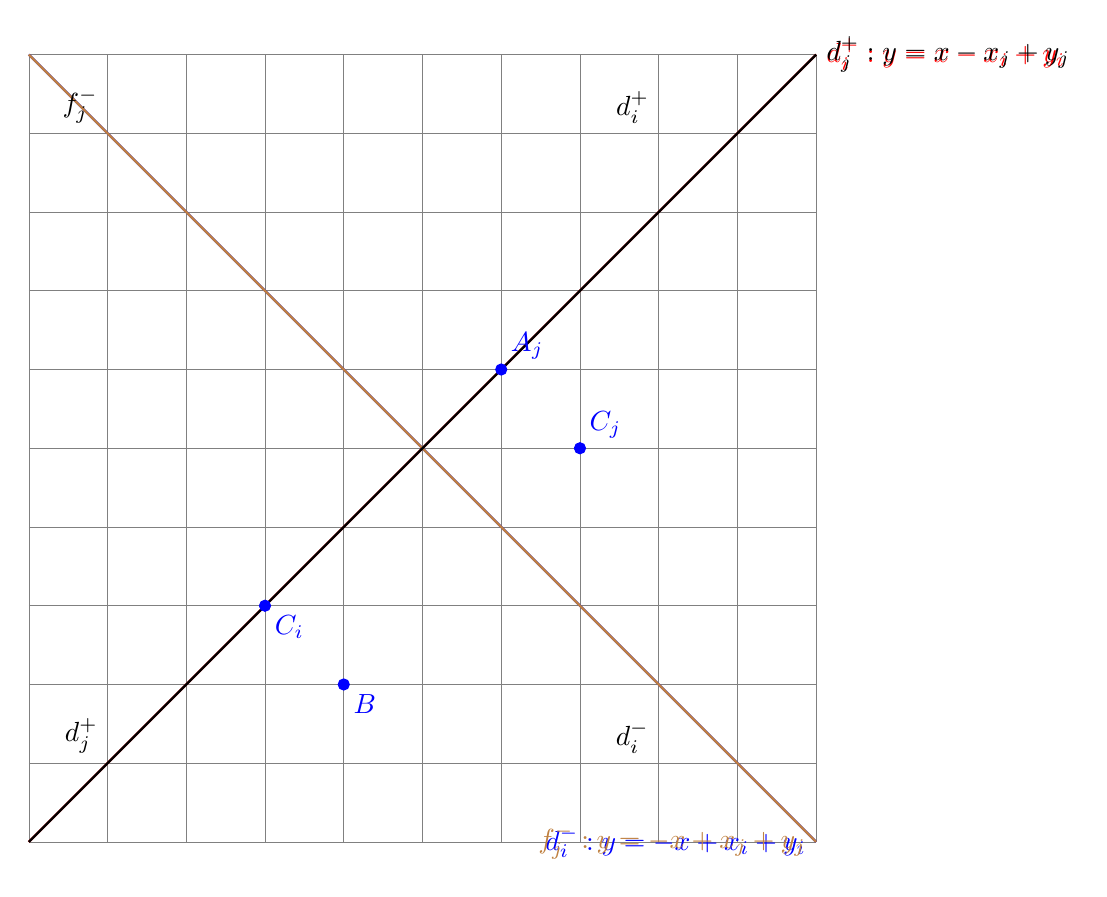
\begin{tikzpicture}[scale=1]
    % Grid
    \draw[help lines] (0,0) grid (10,10);
    
    % Lines
    \draw[red, thick] (0,0) -- (10,10) node[right] {$d_i^+: y = x - x_i + y_i$};
    \draw[blue, thick] (0,10) -- (10,0) node[left] {$d_i^-: y = -x + x_i + y_i$};
    \draw[brown, thick] (0,10) -- (10,0) node[left] {$f_j^-: y = -x + x_j + y_j$};
    \draw[black, thick] (0,0) -- (10,10) node[right] {$d_j^+: y = x - x_j + y_j$};
    
    % Points
    \filldraw[blue] (4,2) circle (2pt) node[below right] {$B$};
    \filldraw[blue] (6,6) circle (2pt) node[above right] {$A_j$};
    \filldraw[blue] (7,5) circle (2pt) node[above right] {$C_j$};
    \filldraw[blue] (3,3) circle (2pt) node[below right] {$C_i$};
    
    % Labels
    \node at (8,9) [above left] {$d_i^+$};
    \node at (1,9) [above left] {$f_j^-$};
    \node at (8,1) [above left] {$d_i^-$};
    \node at (1,1) [above left] {$d_j^+$};
\end{tikzpicture}

\end{document}